% Preamble
% =============================================================================

% Class of the document.
\documentclass[12pt,a4paper]{article}
% article : short article.
% report  : mid-length report.
% book    : book or thesis redaction.

% Paragraph skip length (default to 0).
\setlength{\parskip}{1ex}

% Packages
% =============================================================================

% Encoding
% -----------------------------------------------------------------------------

% Babel.
\usepackage[french]{babel}
% FontEnc.
\usepackage[T1]{fontenc}
% InputEnc.
\usepackage[utf8]{inputenc}

% Define \escapeus command to escape underscores.
\makeatletter
\DeclareRobustCommand*{\escapeus}[1]{
    \begingroup\@activeus\scantokens{#1\endinput}\endgroup}
\begingroup\lccode`\~=`\_\relax
    \lowercase{\endgroup\def\@activeus{\catcode`\_=\active \let~\_}}
\makeatother

% Text
% -----------------------------------------------------------------------------

% Acronym.
\usepackage{acronym}
% CsQuote.
\usepackage[style=french,french=guillemets]{csquotes}
% Enumerate.
\usepackage{enumerate}
% HyperRef.
\usepackage[hyperfootnotes=false,hidelinks]{hyperref}
% URL.
\usepackage{url}

% Algorithms
% -----------------------------------------------------------------------------

% Algorithm2E.
\usepackage[french,onelanguage,linesnumbered,ruled,vlined,commentsnumbered]{algorithm2e}

% Source code
% -----------------------------------------------------------------------------

% Listings.
\usepackage{listings}
% Minted.
\usepackage{minted}
% Caption.
\usepackage{caption}
\newenvironment{code}{\captionsetup{type=listing}}{}

% Files
% -----------------------------------------------------------------------------

% FancyVRB.
\usepackage{fancyvrb}
% Redefine \VerbatimInput.
\RecustomVerbatimCommand{\VerbatimInput}{VerbatimInput}
{
    fontsize=\footnotesize,
    frame=lines,         % Top and bottom rule only.
    framesep=1.5em,      % Separation between frame and text.
    rulecolor=\color{red!50!green!50!blue!50!},
    labelposition=topline,
    commandchars=\|\(\), % Escape character and argument delimiters for commands within the verbatim.
    commentchar=*        % Comment character.
}

% Figures
% -----------------------------------------------------------------------------

% GraphicX.
\usepackage{graphicx}
% SVG.
\usepackage{svg}
% WrapFig.
\usepackage{wrapfig}

% Charts
% -----------------------------------------------------------------------------

% PGFPLots
\usepackage{pgfplots}
\pgfplotsset{compat=1.16}
\usepgfplotslibrary{units}

% Mathematics
% -----------------------------------------------------------------------------

% AmsFonts.
\usepackage{amsfonts}
% AmsMath.
\usepackage{amsmath}
% AmsText.
\usepackage{amstext}
% AmsThm.
\usepackage{amsthm}
\newtheorem{prr}{Propriété}
\newtheorem{pro}{Proposition}
\newtheorem{thm}{Théorème}
\newtheorem{lem}{Lemme}
% NumPrint.
\usepackage{numprint}

% Physics
% -----------------------------------------------------------------------------

% Physics.
\usepackage{physics}

% Presentation
% -----------------------------------------------------------------------------

% XColor.
\usepackage{xcolor}

% References
% -----------------------------------------------------------------------------

% CleveRef.
\usepackage{cleveref}

% Structure.
% -----------------------------------------------------------------------------

% Geometry.
\usepackage{geometry}
% PDFLScape.
\usepackage{pdflscape}
% MultiCol.
\usepackage{multicol}
% TitleSec.
\usepackage{titlesec}
\newcommand{\sectionbreak}{\clearpage} % Use a page break before new sections.
% VMargin.
\usepackage{vmargin}
% FootMisc.
\usepackage[bottom]{footmisc}

% Symbols
% -----------------------------------------------------------------------------

% SIUnitX.
\usepackage{siunitx}

% Table
% -----------------------------------------------------------------------------

% Array.
\usepackage{array}
% BookTabs.
\usepackage{booktabs}
% CSVSimple.
\usepackage{csvsimple}

% Document
% =============================================================================

\begin{document}

\title{Analyse de performance et optimisation de code}
\author{AYOUB Pierre -- BONNAFOUS Camille -- FLAMANT Océane}

\maketitle

\begin{figure}[b]
    \centering
    
\includegraphics[scale=0.3]{figures/isty.jpg}
\end{figure}

\newpage
\begin{abstract}

La simulation numérique est un procédé informatique visant à modéliser un
phénomène par ordinateur, s'agissant le plus souvent d'un phénomène
physique. Cette modélisation prend forme par des systèmes d'équations
décrivant l'état du système physique représenté à chaque instant. De
nombreux domaines scientifiques convergent vers la simulation
informatique, tel que certaines branches de la physique, de l'analyse
et de l'optimisation mathématique, ou encore le calcul haute
performance en informatique. Enfin, la simulation trouve naturellement
de nombreuses applications concernant des sujets variés, tel que la
simulation du climat et des évènements météorologiques, la simulation
d'essais nucléaires, de l'effet d'un médicament sur un corps, ou encore
des astres et de l'univers. Ce rapport s'articulera donc autour de l'analyse et
de l'optimisation d'un code de calcul, coeur des simulations numériques
présentés ci-dessus.

\end{abstract}

\tableofcontents

\section{Introduction}

Le projet que nous vous présentons aujourd'hui consiste à analyser puis,
grâce à nos mesures, optimiser un code de calcul, appelé kernel.

TODO
Afin d'étudier les différents niveaux de mémoires chaque membre du groupe 
analysera un type précis.

\begin{description}
    \item[Pierre] Le cache L1, paramètre de l'ordianteur : 
		\begin{itemize}
				\item TO DO
				\item fréquence
		\end{itemize}
    \item[Océne ] Le cache L2, paramètre de l'ordinateur : 
		\begin{itemize}
			\item cache L1 : 32K,
			\item cache L2 : 256K,
			\item fréquence 2,40GHz
		\end{itemize}
    \item[Camille] La RAM, paramètre de l'ordianteur : 
        \begin{itemize}
			\item TO DO
			\item fréquence
		\end{itemize}
\end{description} 

Le déroulement du projet s'est effectué en plusieurs étapes distinctes :
\begin{description}
    \item[Analyse du code] Cette phase consiste à analyser le programme d'un
        point de vue d'architecture informatique. Il convient d'étudier les
        choix mis en œuvres afin d'implémenter le ou les calculs nécessaires.
    \item[Protocole expérimental] Une fois l'analyse effectuée, nous
        pouvons en déduire le moyen le plus adapté afin de mesurer les
        performances de notre implémentation. Nous allons donc mettre en
        avant les critères théoriques à atteindre dans nos mesures, puis
        nous exposerons la manière dont nous avons mis ceci en pratique.
    \item[Optimisations et mesures] Grâce au protocole mis en place, nous
        pouvons quantifier la performance du programme. De ce fait, nous serons
        en mesure d'expérimenter différentes techniques d'optimisation sur le
        programme et d'en calculer l'accélération.
\end{description}

\section{Analyse du code}

Avant de pouvoir faire toutes les mesures il faut trouver la taille des 
données d'entrée. Pour cela il faut dans un premier connaitre la taille 
de ce dont on a besoin. Dans notre programme nous avons deux tableaux :
\begin{itemize}
    \item un tableau de float à deux dimensions dont la taille en fonction
    de n est 4n*n
    \item un tableau de double à une dimension dont la taille en fonction
    de n est 8n
\end{itemize}

La taille totale de nos données d'entrées est donc 4n*n+8n.

\subsection{Cache L1}
\subsection{Cache L2}
Pour que les deux tableaux entrent entièrement dans le cache L2 il faut 
que la formule respecte les contraintes suivantes : 
\begin{itemize}
    \item la taille totale doit être plus grande que la taille du cache 
    L1 (1); pour plus sécurité il a été décidé que la taille totale devait 
    être au moins trois fois plus grande que celle du L1, 
    \item L2 partage sa mémoire pour stocker à la fois les instructions, 
    les données et ce qui tourne en background on ne peut donc en utiliser 
    que 90\% (2). 
\end{itemize}
Ces deux contraintes peuvent être transformée sous forme d'inéquation :
\begin{itemize}
    \item (1) : 3*TL1<4n*n+8n,
    \item (2) : 4n*n+8n<=0,9*TL2
\end{itemize}
Après la résolution de ces équations on obtient n=156 comme minimum et 
n=242 comme maximum.

\subsection{RAM}



\section{Protocole expérimental}

La mise en place d'un protocole expérimental de mesure est une étape nécessaire
et cruciale dans tout optimisation de code. D'une part, le but de ce protocole
est de mettre en lumière les points chauds du programme, c'est-à-dire les
parties du code qui ralentissent considérablement l'exécution de la simulation.
Ces points chauds seront les cibles de nos optimisations. D'autre part, après
chaque tentative d'optimisation, le protocole doit nous permettre de mesurer
l'impact de cette dernière, qu'il soit positif ou négatif, et enfin de le
quantifier.


TODO



\subsection{Théorie}

Lors de nos expériences, il ne faut pas oublier que le hasard ou l'aléa des
mesures peuvent biaiser un résultat. Afin d'éviter cela, il faut donc utiliser
une valeur moyenne ou une valeur médiane.

\subsubsection{Analyse de sensibilité}

Une fois que l'on connait la taille des données à fourni en entrée, 
il faut faire l'analyse de sensibilité pour les autres paramètres. 
\begin{description}
    \item[Le nombre de métarépétition] Il nous est donné, il est de 31.
    \item[Le nombre de warmup] Il doit se situer entre 1 et 1000. Pour le 
    déterminer il doit être le seul paramètre que l'ont fait varier. On fait 
    plusieurs exections et avec les valeurs obteunues on fait une courbe pour 
    voir à partir de quelle valeur cela devient stable. Il faut aussi vérifier 
    que (médiane-minimum)/minimum est inférieur à 5\%. 
    \item[Le nombre de repetitions] On le trouve de la même manière que 
    le nombre de warmup.
\end{description}


\subsection{Pratique}
Lors de nos première tentatives pour trouver les paramètres nous avons remarqué
que ce qui prenait le plus de temps dans notre noyau était le calcul de 
l'exponentiel. Afin de pouvoir vérifier si nos paramètres sont corrects nous
avons donc modifié le kernel.c pour que ce soit le temps de récupération des
données qui soit le plus grand.

\subsubsection{Cache L1}
TO DO

\subsubsection{Cache L2}
Pour vérifier le calcul théorique de la taille des données j'ai utilisé 
likwid-perftcr afin de voir si les données transitaient bien par le cache L2. 
Après avoir compilé avec gcc uniquement j'ai exécuté l'exécutable avec likwid 
et voici les résultats obtenus :
\newline

\begin{tabular}{|c|c|}
  \hline
  n & Data Volume (GByte) \\
  \hline
  100 & 4,24 \\
  150 & 14,06 \\
  220 & 37,9 \\
  235 & 34,4 \\
  \hline
\end{tabular}

On observe que ces résultats sont en corrélation avec les résultats théoriques
en dessous de 156 pratiquement aucune donnée ne passe par le cache L2 et 
quand on se rapproche de 242 une partie des données ne semble plus passer 
dans L2 je suppose donc que ces données vont directement dans le cache L3.
Au vu de ces informations, j'ai choisi de prendre 220 comme taille de 
données.

\newline
Voici, ci-contre le graphic obtenu pour trouver le bon nombre de warmup. 
On peut observer que le nombre de cycle semble se stabiliser au alentour 
de 100 warmup, Figure 1. Pour plus de sécurité j'ai choisit 150 pour le nombre de 
warmup.

\begin{figure}
    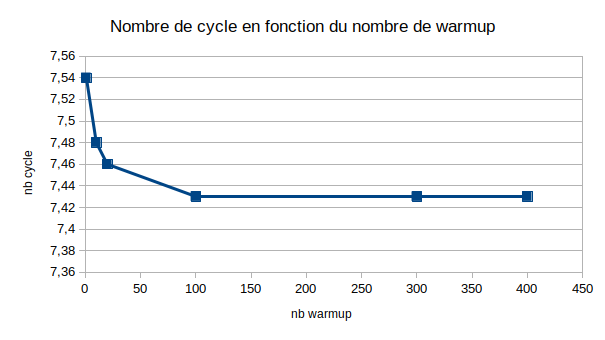
\includegraphics[scale=0.8]{figures/L2/L2warmup.png}
    \caption{Sans l'exponentiel}
\end{figure}

J'ai ensuite vérifié avec le calcul de l'exponetiel et on obtient bien le 
même résultat, Figure 2. 

\begin{figure}
    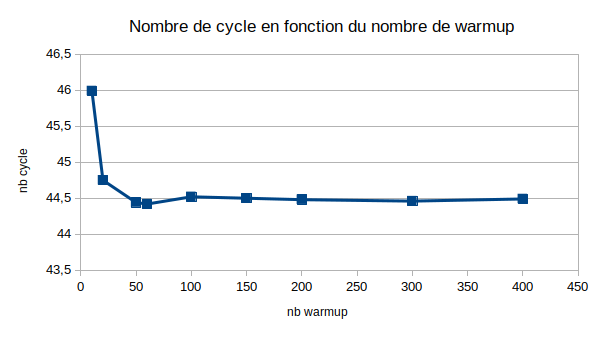
\includegraphics[scale=0.8]{figures/L2/L2warmup2.png}
    \caption{Avec l'exponentiel}
\end{figure}


Pour trouver le bon nombre de répétition j'ai uniquement fait les test avec
l'exponentiel. 
Comme vous pouvez le voir, Figure 3, on peut remarquer que l'ensemble est stable, les
variations sont minimes. J'ai chosit comme nombre de répétition 1200.
\begin{figure}
    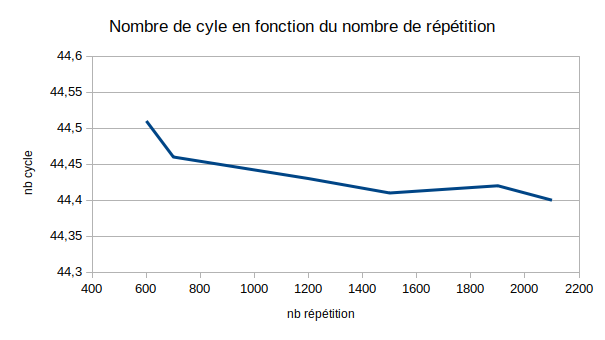
\includegraphics[scale=0.8]{figures/L2/L2repet.png}
    \caption{ }
\end{figure}

\subsubsection{RAM}
TO DO


\section{Optimisations et mesures}

\subsection{Phase 1}
\subsubsection{L1}
\subsubsection{L2}
\subsubsection{RAM}


\subsection{Phase 2}

\section{Conclusion}

TODO


\newpage
\section*{Acronymes}

\begin{acronym}
\end{acronym}

\end{document}
